\chapter{Provedené experimenty}

V této kapitole popíši provedené experimenty a ukáži naměřené výsledky, které následně zhodnotím.

Nejdříve budu hodnotit algoritmy zvlášť v rámci jednotlivých her. V poslední sekci kapitoly zhodnotím testované DDA algoritmy celkově.

Každý z experimentů obsahoval celkem 1000 iterací.

Jednotlivé metriky mají diametrálně odlišné rozsahy hodnot. Z tohoto důvodu v grafech zobrazuji místo konkrétních hodnot poměr k nejlepší hodnotě. Výběr nejlepší hodnoty závisí na druhu metriky. Změnu vedení a svobodu se snažíme maximalizovat, ostatní metriky minimalizujeme. Z tohoto důvodu u změny vedení a svobody zobrazuji poměr vůči maximu, u zbylých metrik je tomu naopak.

Pro jednodušší vizuální porovnávání algoritmů mezi sebou upravuji metriky, které se minimalizují. Pracuji s převrácenou hodnotou těchto metrik. Po této úpravě zobrazuji do grafů poměr k maximální převrácené hodnotě minimalizujících metrik. Z tohoto důvodu čím vyšší hodnoty pro každou z metrik, tím je algoritmus lepší.

\section{Bludiště}

Pro testování bludiště jsem nastavil jeho velikost na šířku a výšku 41 čtverců, maximální počet kroků 777. Koeficienty metrik byly nastaveny na 10 pro uvěřitelnost, 100 pro napětí, 500 pro náskok a 100 pro svobodu. Zbylé koeficienty byly nastaveny na 0. Výsledek si lze prohlédnout na následujícím grafu (\ref{fig-ch5mazehc}) a tabulce(\ref{tab-mazem}).

V grafu jsou použity zkratky pro použité algoritmy. E-HC představuje E-HillClimber, E-MM je pro E-MaxMax, E-MC pro E-MonteCarlo, POSM pro Částečně uspořádaná množina – Mistr a DL pro Dynamickou úroveň. U Bludiště nebyl použit E-MN pro E-Max$^n$. Algoritmus E-Max$^n$ má za úkol simulovat hráče. Hráč ve hře bludiště se rozhoduje pouze dle následujících stavů. Z tohoto důvodu zde je postačující Algoritmus E-MaxMax, který plní přesně stejnou funkci jako E-Max$^n$ u dalších her. Algoritmus Žádný představuje naměřené metriky z hry, kdy nebyl použit žádný DDA mechanismus. Slouží pro srovnání s DDA algoritmy.

\begin{figure}
  \centering
  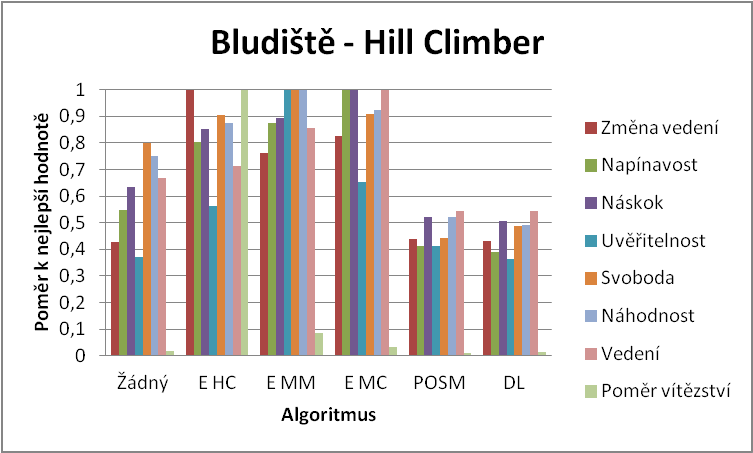
\includegraphics[width=0.75\textwidth]{ch5mazehc}
	\caption{Srovnání DDA alg. ve hře Bludiště s Hill Climber hráčem.}
	\label{fig-ch5mazehc}
\end{figure}

Z tabulky a především z grafu lze vyčíst, že algoritmy POSM a DL zaostávají nejen za ostatními DDA algoritmy, ale také za hrou, kde není použit žádný DDA mechanismus. Dopadají hůře i v metrikách napínavost a náskok, na kterých je testovali jejich autoři.

Při bližším zkoumání jsem zjistil, že důvodem pro špatné chování je absence přizpůsobování se metrice svoboda. Oba algoritmy příliš ořezávají možné tahy hráče na průměrných 7 tahů během hry. Bez použití DDA je průměrná hodnota svobody 12. Při nízké svobodě má hráč ve hře malé množství dveří, kterými by se vydal. Ve hře existuje málo větvení a naopak dlouhé chodby. Z tohoto důvodu se hráči rychle snižuje neprobádaný prostor - dlouhé chodby bez postranních dveří často odříznou část mapy od hráče. 

Oba algoritmy pracují pouze s hloubkou 1 a často se dostanou do situace, kdy už musí vytvořit chodbu k poslední bombě, přestože hráči zbývá ještě dostatek času. Případně nastane zcela opačná situace. Na mapě je více jak jedna bomba, tedy tyto algoritmy mohou bombu, ke které směřuje hráč, odříznout a udělat z ní falešnou, ale jelikož jsou ve hře především dlouhé nevětvené chodby, hráč se musí vrátit o velké množství kroků a vyprší mu čas.

\begin{table*}[b]\footnotesize
\vspace*{0mm}
\caption{{\label{tab-mazem}} Porovnání metrik zábavnosti u jednotlivých algoritmů ve hře Bludiště. Metriky změna vedení a svoboda se maximalizují, zbytek minimalizuje.}
\vspace*{0mm}
\label{shadowtable}
\begin{center}
\begin{tabular}{| l || r | r | r | r | r | r | r | r | r | r |}
\hline
Algoritmus & Počet kol	& Změna vedení & Napínavost & Náskok & Uvěřitelnost\\
\hline
\hline
Žádný & 93,127 & 8,217 & 343,6848421 & 239,851 & 81789,7937 \\ \hline  
E-HC & 114,905 & 19,176 & 233,9169735 & 177,951 & 53868,86 \\ \hline
E-MM & 113,32 & 14,64 & 214,5392914 & 169,935 & 30377,59274 \\ \hline
E-MC & 105,494 & 15,829 & 187,5847573 & 151,923 & 46656,61097 \\ \hline
POSM & 99,902 & 8,394 & 455,7661817 & 290,602 & 73884,68107 \\ \hline
DL & 95,431 & 8,29 & 483,7274291 & 300,486 & 83988,2358 \\ \hline
\end{tabular}
\end{center}
\begin{center}
\begin{tabular}{| l || r | r | r | r | r | r | r | r | r |}
\hline
Algoritmus & Svoboda & Náhodnost & Vedení &	Rozptyl Vítězů \\
\hline
\hline
Žádný & 12,19857537 & 15,05552294 & 33,04804979 & 0,121 \\ \hline  
E-HC & 13,79978394 & 12,92183276 & 31,00734155 & 0,002 \\ \hline
E-MM & 15,26174269 & 11,29628595 & 25,74151376 & 0,024 \\ \hline
E-MC & 13,84465841 & 12,22155687 & 22,05607333 & 0,065 \\ \hline
POSM & 6,76593984 & 21,72255666 & 40,54974306 & 0,176 \\ \hline
DL & 7,45030571 & 22,91638791 & 40,45994322 & 0,154 \\ \hline
\end{tabular}
\end{center}
\end{table*}

Algoritmy E-HC, E-MM a E-MC dopadly obdobně. Algoritmu E-HC se nejlépe dařilo v metrikách poměr vítězství a změna vedení, E-MM zvítězil v uvěřitelnosti, náhodnosti a svobodě, E-MC dopadl nejlépe v napínavosti, náskoku a ve vedení. Celkově nejlépe si vedl v této hře algoritmus E-MaxMax.

\subsection{Vzhled bludiště pro různé DDA algoritmy}

Druh použitého DDA algoritmu má velký vliv na výsledný vzhled bludiště. Typické zástupce vytvořených bludišť ukazuje obr. \ref{fig-mazes}. Pro bludiště vytvořené náhodně jsou typické zpočátku dlouhé chodby a posléze vyplňování chodbiček mezi dlouhými chodbami. Z vlastních algoritmů jsem vybral zástupce E-MaxMax, jehož bludiště působí nejpřirozeněji.

\begin{figure}
  \centering
  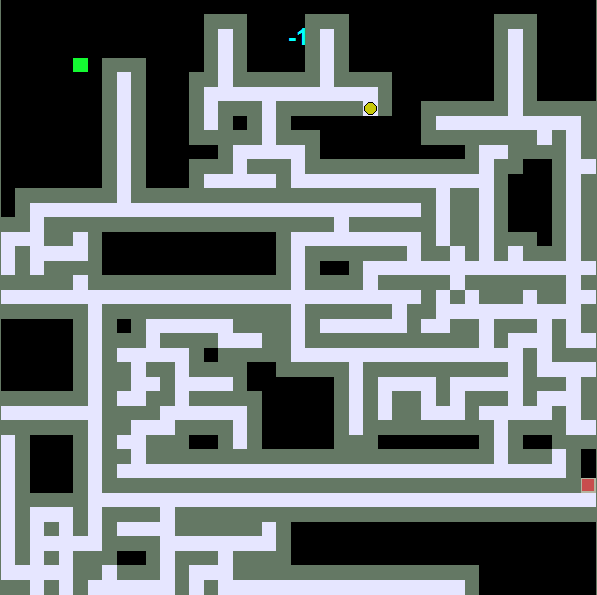
\includegraphics[width=0.35\textwidth]{mzadny}
	\hspace{3pt}
	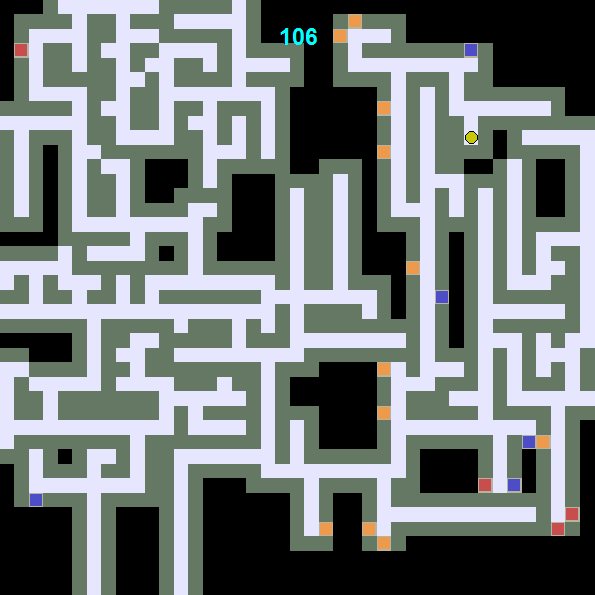
\includegraphics[width=0.35\textwidth]{mmaxmax} \\
	\vspace{6pt}
	\includegraphics[width=0.35\textwidth]{mposm}
	\hspace{3pt}
	\includegraphics[width=0.35\textwidth]{mdl}
	\caption{Srovnání bludišť vytvořených různými DDA algoritmy. Zleva-doprava, shora-dolů: žádný, E-MaxMax, POSM, DL}
	\label{fig-mazes}
\end{figure}

Bludiště vytvořená pomocí POSM a DL vypadají obdobně. Je pro ně typický výrazný počáteční kříž chodeb, kde algoritmy brzy uzavřou tři možné cesty a nechají mu jednu poslední.

\section{Ludo}

Oproti hře Bludiště je ve hře Ludo zásadní metrikou uvěřitelnost. V případě, že na tuto metriku nedáme důraz, HP nedovolí žádnému z hráčů hru vyhrát. Z jeho pohledu je ideální, když všichni hráči mají 3 figury v cíli a 4 těsně před cílem. Tato situace se mu zdá napínavá a ona by i ve skutečné hře byla, ale ne v případě použití falešné kostky. Z tohoto důvodu jsem nastavil koeficienty u uvěřitelnosti na 1000, spravedlnost, vedení, napětí na 10, náskok na 3 a svobodu na 1.

S tímto nastavením jsem provedl 3 experimenty. V prvních dvou hráli pouze dva hráči, jednou s algoritmem Hill Climber, podruhé s Max$^n$. Experiment s dvěma hráči jsem spouštěl, aby měly algoritmy Dynamický level a POSM prostředí, pro které byly navrhnuty - dvouhráčové hry. V třetí experimentu byly 4 hráči Max$^n$. První měl úroveň 50, další tři 100. Pro test DL a POSM jsem nahradil všechny 3 poslední hráče právě algoritmy DL, nebo POSM.

\begin{figure}
  \centering
  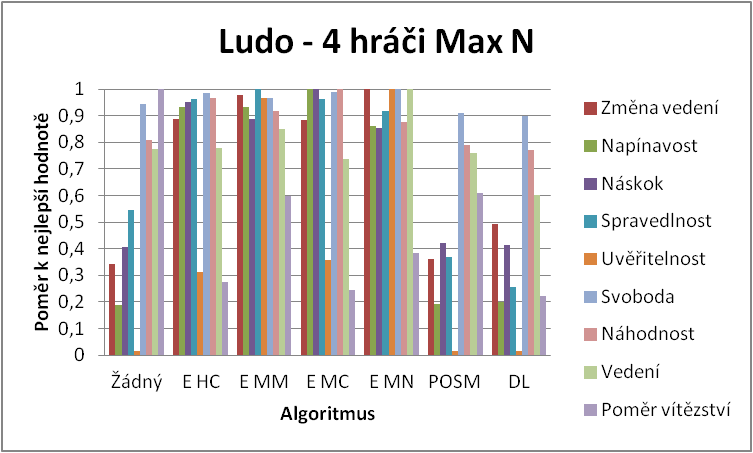
\includegraphics[width=0.75\textwidth]{ch5ludo4maxn}
	\caption{Srovnání DDA alg. ve hře Ludo se 4 Max$^n$ hráči. (úrovně 50, 100, 100, 100)}
	\label{fig-ch5ludo4maxn}
\end{figure}

Výsledky všech 3 experimentů byly obdobné. Zde uvedu pouze graf(\ref{fig-ch5ludo4maxn}) a tabulku(\ref{tab-ludom}) posledního experimentu. Grafy zbylých dvou experimentů lze nalézt v příloze.

\begin{table*}[b]\footnotesize
\vspace*{0mm}
\caption{{\label{tab-ludom}} Porovnání metrik zábavnosti u jednotlivých algoritmů ve hře Ludo. Metriky změna vedení a svoboda se maximalizují, zbytek minimalizuje.}
\vspace*{0mm}
\label{shadowtable}
\begin{center}
\begin{tabular}{| l || r | r | r | r | r | r | r | r | r | r |}
\hline
Algoritmus & Počet kol	& Změna vedení & Napínavost & Náskok & Spravedlnost\\
\hline
\hline
Žádný & 321,629 & 33,207 & 10,96064284 & 10,69 & 0,053439508 \\ \hline  
E-HC & 367,71 & 86,401 & 2,191965172 & 4,576 & 0,030182817 \\ \hline  
E-MM & 374,831 & 95,074 & 2,197616324 & 4,911 & 0,029112477 \\ \hline  
E-MC & 370,011 & 86,126 & 2,047674062 & 4,351 & 0,030268374 \\ \hline  
E-MN & 349,386 & 97,275 & 2,378575689 & 5,096 & 0,031668999 \\ \hline  
POSM & 329,262 & 35,024 & 10,57217622 & 10,292 & 0,079106286 \\ \hline  
DL & 342,281 & 47,836 & 10,26501397 & 10,484 & 0,113375705 \\ \hline  
\end{tabular}
\end{center}
\begin{center}
\begin{tabular}{| l || r | r | r | r | r | r | r | r | r |}
\hline
Algoritmus & Uvěřitelnost & Svoboda & Náhodnost & Vedení &	Poměr vítězství \\
\hline
\hline
Žádný & 24,57354378 & 1,86791164 & 1,189324764 & 67,3734372 & 0,021365861 \\ \hline  
E-HC & 1,226482879 & 1,95087896 & 0,996415593 & 67,020713 & 0,078176083 \\ \hline  
E-MM & 0,396586046 & 1,90887509 & 1,047952319 & 61,58128218 & 0,035686132 \\ \hline  
E-MC & 1,078624424 & 1,95431191 & 0,963174893 & 70,7910895 & 0,087272562 \\ \hline  
E-MN & 0,383798925 & 1,9757931 & 1,100121925 & 52,281059 & 0,055709066 \\ \hline  
POSM & 25,21722299 & 1,79829072 & 1,216838264 & 68,67222926 & 0,035035696 \\ \hline  
DL & 26,54645197 & 1,77747205 & 1,250394015 & 86,85364229 & 0,096187317 \\ \hline  
\end{tabular}
\end{center}
\end{table*}

Algoritmy POSM a DL měly zde již svou tradiční úlohu - ovládaly běžné hráče. Z tohoto důvodu neovlivňovaly metriky uvěřitelnost, svoboda, náhodnost a spravedlnost, které musely dopadnout podobně jako při nepoužití žádného DDA algoritmu. Oba zlepšily metriku změny vedení, ale zhoršily poměr vítězství. Náskok i napínavost měly podobnou, jako by se žádné DDA nepoužilo. 

U této hry a ještě více u Ztracených měst se projevil zásadní problém těchto DDA mechanismů. Pokud hráči jimi ovládaní jsou ve vedení, zhoršují svoje chování. Zhoršují ho až do zcela iracionální podoby. U hry Ludo se iracionální chování projeví např. v situaci, kdy hráč má jednu figurku před cílem a na kostce padla správná hodnota, aby hráč mohl přesunout svou figurku do cíle. V případě, že je hráč již dlouho ve vedení, tak raději nechá v figurku v potencionálně nebezpečné pozici a pohne figurkou jinou. 

Algoritmy E-HC, E-MM, E-MC a E-MN velmi předčily zbytek algoritmů i v metrice uvěřitelnost. V případě náhodného chování kostky se může s malou pravděpodobností stát, že padne jednomu hráči 6 třikrát po sobě. Je to relativně málo pravděpodobné, ale stát se to může. Algoritmy HP se snaží tyto málo pravděpodobné jevy eliminovat, a proto si dle metriky uvěřitelnost vedly lépe.

Celkově si nejlépe vedly E-MM a E-MN, které dokáží celkem věrně simulovat chování hráčů a následně se rozhodovat dle stavů hry dále v budoucnu. Mohou lépe naplánovat chování kostky z hlediska uvěřitelnosti a díky tomu se zaměřit více na ostatní metriky.

\section{Ztracená města}

I u Ztracených měst byla nejdůležitější metrikou uvěřitelnost. Bez ní prohrávající hráč získával postupně karty hodnot 10, 9, 8 atd. barev již vyložených expedic, dokud se nedostal do vedení. Nastavení koeficientů metrik jsem zvolil 1000 pro uvěřitelnost, 100 pro změnu vedení, spravedlnost, vedení a napětí, 10 pro svobodu a 0 pro náskok.

\begin{table*}[b]\footnotesize
\vspace*{0mm}
\caption{{\label{tab-lcm}} Porovnání metrik zábavnosti u jednotlivých algoritmů ve hře Ztracená města. Metriky změna vedení a svoboda se maximalizují, zbytek minimalizuje.}
\vspace*{0mm}
\label{shadowtable}
\begin{center}
\begin{tabular}{| l || r | r | r | r | r | r | r | r | r | r |}
\hline
Algoritmus & Počet kol	& Změna vedení & Napínavost & Náskok & Spravedlnost\\
\hline
\hline
Žádný & 51,21 & 5,17 & 169,3785106 & 159,11 & 2,97949985 \\ \hline  
E-HC & 51,652 & 6,219 & 90,11489792 & 109,66 & 2,083795471 \\ \hline  
E-MM & 51,058 & 15,105 & 35,89171719 & 92,52 & 2,51490921 \\ \hline  
E-MC & 51,076 & 6,763 & 84,52874032 & 106,63 & 2,407272356 \\ \hline  
E-MN & 51,284 & 16,647 & 34,66283799 & 78,3 & 1,853999951 \\ \hline  
POSM & 53,785 & 5,038 & 204,2092341 & 217,97 & 3,458477317 \\ \hline  
DL & 49,957 & 4,838 & 283,7280003 & 228,54 & 3,401727139 \\ \hline  
\end{tabular}
\end{center}
\begin{center}
\begin{tabular}{| l || r | r | r | r | r | r | r | r | r |}
\hline
Algoritmus & Uvěřitelnost & Svoboda & Náhodnost & Vedení &	Poměr vítězství \\
\hline
\hline
Žádný & 4,930532754 & 30,0635238 & 12,59686374 & 15,751 & 0,016 \\ \hline  
E-HC & 0,612039822 & 31,8330098 & 10,61479482 & 15,426 & 0,055 \\ \hline  
E-MM & 0,467313632 & 29,8150478 & 11,6301367 & 6,802 & 0,093 \\ \hline  
E-MC & 0,78408408 & 31,6226395 & 11,05890933 & 14,119 & 0,089 \\ \hline  
E-MN & 0,52395678 & 29,1162948 & 11,52272589 & 7,209 & 0,081 \\ \hline  
POSM & 4,956223714 & 27,4061938 & 12,97565858 & 16,7575 & 0,358 \\ \hline  
DL & 4,944157754 & 26,5193542 & 14,25249958 & 18,3885 & 0,408 \\ \hline  
\end{tabular}
\end{center}
\end{table*}

Opět byly spuštěny dva experimenty s různými v hráči. V jednom hráli proti sobě HillClimber IS s úrovněmi 50 a 100 a v druhém MiniMax IS se stejnými úrovněmi. Výsledky byly podobné, a proto se zaměřím na experiment se složitějšími hráči (graf \ref{fig-ch5lcmm}, tabulka \ref{tab-lcm}). Graf druhého experimentu lze nalézt v příloze.

DL a POSM opět ovládaly jednoho z hráčů, a tedy nemohly ovlivnit čtveřici metrik spravedlnost, uvěřitelnost, svoboda a náhodnost. Oba dva algoritmy dopadly špatně z důvodu nastíněného u hry Ludo. Ve Ztracených městech člověk dokáže snadno rozlišit zcela iracionální tahy od těch použitelných. DL a POSM ale mají tyto iracionální tahy k dispozici. Jestliže je hráč ovládaný DL nebo POSM ve vedení, nejrychleji srovná skóre vyložením nové expedice, za kterou má záporné body. Bohužel takový tah může být zásadní a i kdyby posléze hrál daný hráč dokonale, nemusí mu to stačit k opětovnému dostání se do vedení. Z tohoto důvodu je u Ztracených měst lepší nepoužít žádný algoritmus než POSM a DL v nezměněné podobě.

\begin{figure}
  \centering
  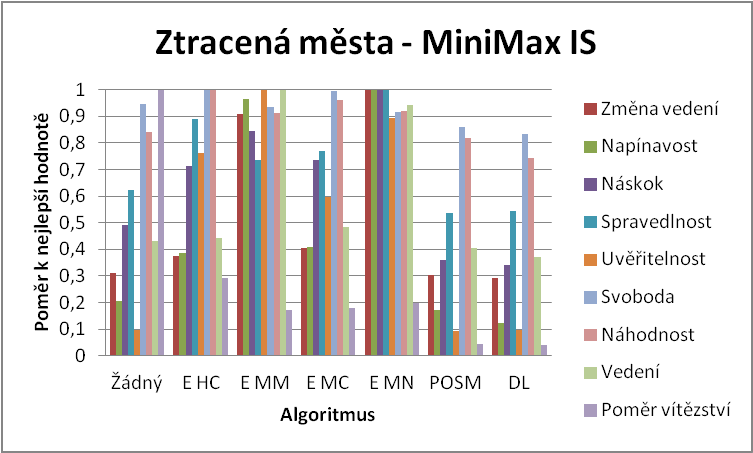
\includegraphics[width=0.75\textwidth]{ch5lcmm}
	\caption{Srovnání DDA alg. ve hře Ztracená Města s dvěma MiniMax IS hráči. (úrovně 50 a 100)}
	\label{fig-ch5lcmm}
\end{figure}

E-MC a E-HC dopadly navzájem podobně, ale oba lépe než hra bez DDA. Jelikož E-HC je znatelně rychlejší, je v tomto případě vhodnější než E-MC. Vítězem u Ztracených měst je jednoznačně E-MN, který byl nejlepší v metrikách změna vedení, napínavost, náskok a spravedlnost.

\section{Celkové srovnání}

Pro celkové srovnání použitých DDA algoritmů jsem každý algoritmus ohodnotil v jednotlivých hrách na základě všech 9 metrik a zvlášť na základě pouze 4 metrik změna vedení, napětí, náskok a poměr vítězství. Dvojí hodnocení jsem použil ze dvou důvodů. Algoritmy POSM a DL nebyly navrženy pro testování na daných metrikách a za druhé jejich použití u her Ludo a Ztracená města neovlivňuje 4 ze zbylých metrik.

Hodnocení algoritmu ve hře se rovná součtu hodnocení za jednotlivé metriky. Algoritmus, který si vedl nejlépe v daném metrice, získal celý bod za tuto metriku. Ostatní algoritmy si přičetly poměr jejich hodnoty k nejlepší hodnotě. Z toho vyplývá, že u prvního hodnocení je maximální hodnota 9, u druhého 4.

\begin{figure}
  \centering
  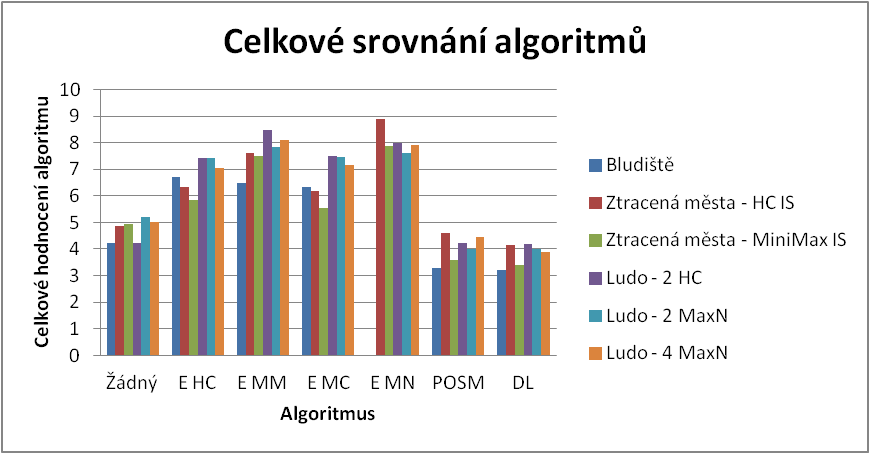
\includegraphics[width=0.80\textwidth]{ch5all}
	\caption{ Srovnání alg. DDA na základě všech experimentů a metrik. }
	\label{fig-ch5all}
\end{figure}

První hodnocení je znázorněno na grafu \ref{fig-ch5all} a v tabulce \ref{tab-all8m}. Nejlépe dopadly algoritmy E-MM a E-MN. E-MN získal ve Ztracených městech téměř maximální počet 9 bodů, získal 8,87. Za nimi následuje dvojice E-HC a E-MC se zisky kolem 6,5 bodů. DL s POSM dopadly nejhůře se zisky kolem 4 bodů.

\begin{table*}[b]\footnotesize
\vspace*{0mm}
\caption{{\label{tab-all8m}} Celkové hodnocení algoritmů v 6 experimentech na základě 9 metrik.}
\vspace*{0mm}
\label{shadowtable}
\begin{center}
\begin{tabular}{| l || r | r | r | r | r | r | r | r | r |}
\hline
Algoritmus & Bludiště & ZM-HC IS & ZM-MM IS & Ludo-2HC & Ludo-2MN & Ludo-4MN \\
\hline
\hline
Žádný & 4,21 & 4,88 & 4,94 & 4,23 & 5,22 & 5,03\\ \hline  
E-HC & 6,71 & 6,35 & 5,86 & 7,40 & 7,43 & 7,06\\ \hline  
E-MM & 6,47 & 7,62 & 7,48 & 8,47 & 7,85 & 8,10\\ \hline  
E-MC & 6,34 & 6,20 & 5,53 & 7,50 & 7,46 & 7,18\\ \hline  
E-MN & Neměřeno & 8,87 & 7,87 & 8,00 & 7,61 & 7,89\\ \hline  
POSM & 3,30 & 4,59 & 3,59 & 4,23 & 4,00 & 4,43\\ \hline  
DL & 3,23 & 4,14 & 3,38 & 4,20 & 3,99 & 3,87\\ \hline  
\end{tabular}
\end{center}
\end{table*}

Zaměříme-li se pouze na 4 zmíněné metriky, dojde ke stejným závěrům. Zajímavostí je, že ve hře Ztracená města s dvěma HillClimber hráči algoritmus E-MN dominoval ve všech 4 metrikách. DL a POSM i zde sbírají poslední místa.

Oba tyto algoritmy byly navrženy a testovány u her, kde jeden špatný tah zpravidla nerozhodne hru - testovanými hrami byl backgammon u DL a dáma s čínskými šachy u POSM.

\begin{figure}
  \centering
  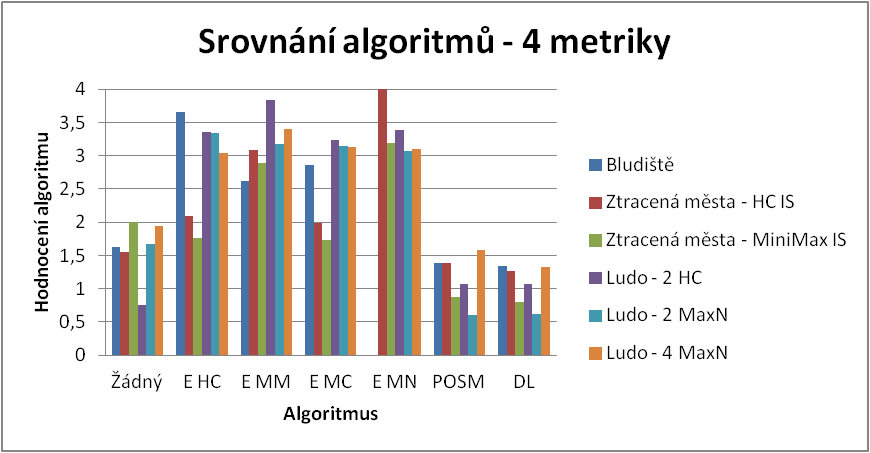
\includegraphics[width=0.80\textwidth]{ch5all4m}
	\caption{ Srovnání alg. DDA na základě všech experimentů a metrik Změna vedení, Napětí, Náskok a Poměr vítězů. }
	\label{fig-ch5all4m}
\end{figure}

Vzhledem výsledkům lze říci, že v případě dostatku výpočetního času a znalosti možných tahů hráčů, je nejvhodnější využít jeden z algoritmů E-MaxMax, nebo E-Max$^n$. Algoritmus založený na Monte Carlo prohledávání stromu dopadá obdobně jako E-HillClimber, ale má mnohem větší časovou náročnost a též potřebuje znalost možných tahů, a tedy se neukázal jako doporučitelný. E-HillClimber sice zaostává za první zmíněnou dvojicí, ale ne o moc. Průměrně dosáhl výsledku 6,8 bodů, E-MaxMax 7,7 a E-Max$^n$ 8,1. Z důvodu jednoduché implementace algoritmu a dobrým výsledkům může být E-HillClimber velice vhodným kandidátem na požití pro techniky DDA ve velikém spektru aplikací. Algoritmy dynamická úroveň a POSM se neukázaly být vhodné pro použití u tohoto typu her.

Pro doplnění E-MonteCarlo dosáhlo průměrně 6,7 bodů, POSM 4,0 a DL 3,8. Bez DDA se dosáhlo 4,8 bodů.

\begin{table*}[b]\footnotesize
\vspace*{0mm}
\caption{{\label{tab-all4m}} Celkové hodnocení algoritmů v 6 experimentech na základě 4 metrik - změna vedení, napínavost, náskok a poměr vítězství.}
\vspace*{0mm}
\label{shadowtable}
\begin{center}
\begin{tabular}{| l || r | r | r | r | r | r | r | r | r |}
\hline
Algoritmus & Bludiště & ZM-HC IS & ZM-MM IS & Ludo-2HC & Ludo-2MN & Ludo-4MN \\
\hline
\hline
Žádný & 1,62 & 1,54 & 2,01 & 0,76 & 1,67 & 1,94\\ \hline  
E-HC & 3,66 & 2,09 & 1,76 & 3,36 & 3,34 & 3,05\\ \hline  
E-MM & 2,62 & 3,09 & 2,89 & 3,83 & 3,18 & 3,39\\ \hline  
E-MC & 2,86 & 1,99 & 1,73 & 3,24 & 3,15 & 3,13\\ \hline  
E-MN & Neměřeno & 4,00 & 3,20 & 3,38 & 3,07 & 3,10\\ \hline  
POSM & 1,38 & 1,39 & 0,88 & 1,07 & 0,60 & 1,59\\ \hline  
DL & 1,34 & 1,27 & 0,79 & 1,08 & 0,62 & 1,33 \\ \hline  
\end{tabular}
\end{center}
\end{table*}

\endinput
%%
%% End of file `ch01.tex'.
